\documentclass{beamer}
%
% Choose how your presentation looks.
%
% For more themes, color themes and font themes, see:
% http://deic.uab.es/~iblanes/beamer_gallery/index_by_theme.html
%
\mode<presentation>
{
  \usetheme{Madrid}      % or try Darmstadt, Madrid, Warsaw, ...
  \usecolortheme{seahorse} % or try albatross, beaver, crane, ...
  \usefonttheme{serif}  % or try serif, structurebold, ...
  \setbeamertemplate{navigation symbols}{}
  \setbeamertemplate{caption}[numbered]
} 

\usepackage[english]{babel}
\usepackage{kotex}
\usepackage{tikz}
\usepackage{listings}
\usepackage{pgffor}
\usepackage{listings}
\usepackage{amsfonts}
\usepackage[linesnumbered,ruled,vlined]{algorithm2e}
\usepackage{algorithmic}

% algorithmbis environment
\makeatletter
\newcounter{algorithmbis}[section]
\setcounter{algorithmbis}{0}
\renewcommand{\thealgorithmbis}{\arabic{algorithmbis}}
\def\algorithmbis{\@ifnextchar[{\@algorithmbisa}{\@algorithmbisb}}
\def\@algorithmbisa[#1]{%
  \refstepcounter{algorithmbis}
  \trivlist
  \leftmargin\z@
  \itemindent\z@
  \labelsep\z@
  \item[\colorbox{lightgray}{\parbox{\textwidth}{%
	    \noindent\strut\textbf{\sf\small 코드 \sf\small\thealgorithmbis} \sf\small#1}
  }]\hfil\vskip0em%
  \color{darkgray}
}
\def\@algorithmbisb{\@algorithmbisa[]}
\def\endalgorithmbis{\hfil\endtrivlist}
\makeatother

\lstset{ %
  backgroundcolor=\color{white},   % choose the background color; you must add \usepackage{color} or \usepackage{xcolor}
  basicstyle=\footnotesize,        % the size of the fonts that are used for the code
  breakatwhitespace=false,         % sets if automatic breaks should only happen at whitespace
  breaklines=true,                 % sets automatic line breaking
  captionpos=b,                    % sets the caption-position to bottom
  commentstyle=\color{gray},    % comment style
  deletekeywords={...},            % if you want to delete keywords from the given language
  escapeinside={\%*}{*)},          % if you want to add LaTeX within your code
  extendedchars=true,              % lets you use non-ASCII characters; for 8-bits encodings only, does not work with UTF-8
  frame=single,                    % adds a frame around the code
  keepspaces=true,                 % keeps spaces in text, useful for keeping indentation of code (possibly needs columns=flexible)
  keywordstyle=\color{blue},       % keyword style
  language=C++,                 % the language of the code
  morekeywords={*,...},            % if you want to add more keywords to the set
  numbers=left,                    % where to put the line-numbers; possible values are (none, left, right)
  numbersep=5pt,                   % how far the line-numbers are from the code
  numberstyle=\tiny\color{gray}, % the style that is used for the line-numbers
  rulecolor=\color{black},         % if not set, the frame-color may be changed on line-breaks within not-black text (e.g. comments (green here))
  showspaces=false,                % show spaces everywhere adding particular underscores; it overrides 'showstringspaces'
  showstringspaces=false,          % underline spaces within strings only
  showtabs=false,                  % show tabs within strings adding particular underscores
  stepnumber=1,                    % the step between two line-numbers. If it's 1, each line will be numbered
  stringstyle=\color{gray},     % string literal style
  tabsize=2,                       % sets default tabsize to 2 spaces
  title=\lstname                   % show the filename of files included with \lstinputlisting; also try caption instead of title
}

\title[3D 그래픽스 프로그래밍]{그래픽스 강의노트 07 - 조명 2 (메시)}
\author{강영민}
\institute{동명대학교}
\date{2015년 2학기}

\begin{document}

%%%%%%%%%%%%%%%%%%%%%%%%%%%%%%%%%%%%%%%%%%%%%%%%%%%%%%%%%
\begin{frame}
  \titlepage
\end{frame}

% Uncomment these lines for an automatically generated outline.
%\begin{frame}{Outline}
%  \tableofcontents
%\end{frame}




%%%%%%%%%%%%%%%%%%%%%%%%%%%%%%%%%%%%%%%%%%%%%%%%%%%%%%%%%
\begin{frame}[fragile]{법선의 설정과 메시(mesh) 데이터 그리기}

\begin{itemize}
\item 앞서 그려본 주전자는 그려지는 면의 법선 벡터가 내장되어 있는 {\sf glutSolidTeapot} 함수를 호출
\item 임의의 면을 그릴 때는 이러한 미리 정의된 법선 벡터가 존재하지 않음
\item 퐁 쉐이딩의 계산이 요구되는 법선 벡터를 오픈지엘에 넘겨주어야 함
\end{itemize}

\end{frame}
%%%%%%%%%%%%%%%%%%%%%%%%%%%%%%%%%%%%%%%%%%%%%%%%%%%%%%%%%



%%%%%%%%%%%%%%%%%%%%%%%%%%%%%%%%%%%%%%%%%%%%%%%%%%%%%%%%%
\begin{frame}[fragile]{구로(Gouraud) 세이딩}

\begin{itemize}
\item 각 정점에 법선 벡터 정의
\item 법선 벡터와 조명의 관계를 이용하여 정점별 퐁 쉐이딩
\item 정점의 색을 이용하여 내부의 픽셀은 선형보간(linear interpolation)을 통해 얻음
\end{itemize}

\begin{figure}[h!]
  \centering
    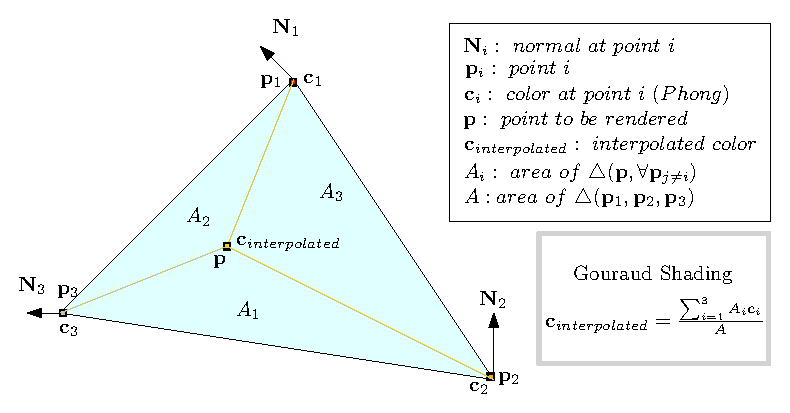
\includegraphics[height=5cm]{OGL_light/interpolatedColors.eps}
\end{figure}
\end{frame}
%%%%%%%%%%%%%%%%%%%%%%%%%%%%%%%%%%%%%%%%%%%%%%%%%%%%%%%%%

%%%%%%%%%%%%%%%%%%%%%%%%%%%%%%%%%%%%%%%%%%%%%%%%%%%%%%%%%
\begin{frame}[fragile]{구로(Gouraud) 세이딩}

\begin{itemize}
\item 각 정점에 법선 벡터 정의
\item 법선 벡터와 조명의 관계를 이용하여 정점별 퐁 쉐이딩
\item 정점의 색을 이용하여 내부의 픽셀은 선형보간(linear interpolation)을 통해 얻음
\end{itemize}

\begin{figure}[h!]
  \centering
    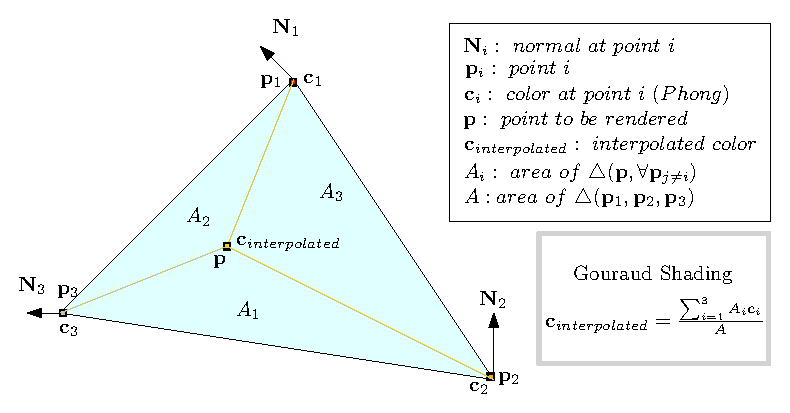
\includegraphics[height=5cm]{OGL_light/interpolatedColors.eps}
\end{figure}
\end{frame}
%%%%%%%%%%%%%%%%%%%%%%%%%%%%%%%%%%%%%%%%%%%%%%%%%%%%%%%%%

%%%%%%%%%%%%%%%%%%%%%%%%%%%%%%%%%%%%%%%%%%%%%%%%%%%%%%%%%
\begin{frame}[fragile]{구로(Gouraud) 세이딩}

\begin{itemize}
\item 각 정점에 법선 벡터 정의
\item 법선 벡터와 조명의 관계를 이용하여 정점별 퐁 쉐이딩
\item 정점의 색을 이용하여 내부의 픽셀은 선형보간(linear interpolation)을 통해 얻음
\end{itemize}

\begin{figure}[h!]
  \centering
    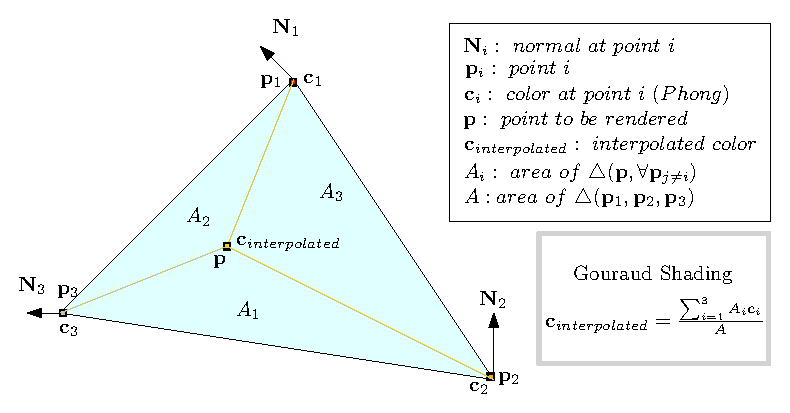
\includegraphics[height=5cm]{OGL_light/interpolatedColors.eps}
\end{figure}
\end{frame}
%%%%%%%%%%%%%%%%%%%%%%%%%%%%%%%%%%%%%%%%%%%%%%%%%%%%%%%%%

%%%%%%%%%%%%%%%%%%%%%%%%%%%%%%%%%%%%%%%%%%%%%%%%%%%%%%%%%
\begin{frame}[fragile]{구로(Gouraud) 세이딩 예제}

\begin{figure}[h!]
  \centering
    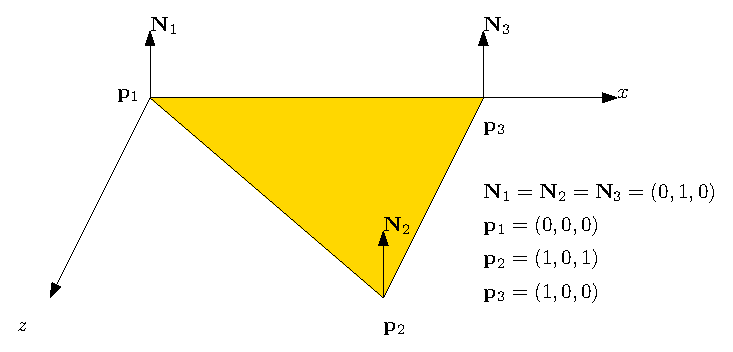
\includegraphics[height=6cm]{OGL_light/simpleTriangle.eps}
\end{figure}

\end{frame}
%%%%%%%%%%%%%%%%%%%%%%%%%%%%%%%%%%%%%%%%%%%%%%%%%%%%%%%%%

%%%%%%%%%%%%%%%%%%%%%%%%%%%%%%%%%%%%%%%%%%%%%%%%%%%%%%%%%
\begin{frame}[fragile]{구로 세이딩을 위한 코딩}

\lstset{language=C++, escapechar=^} 
\begin{lstlisting}
\begin{lstlisting}
  glBegin(GL_TRIANGLES);
  glNormal3f(0,1,0);
  glVertex3f(0,0,0);
  glNormal3f(2/sqrt(3),1/sqrt(3),0);
  glVertex3f(2,0,0);
  glNormal3f(-2/sqrt(3),1/sqrt(3),0);
  glVertex3f(1,0,-1);
  glEnd();
\end{lstlisting}

\end{frame}
%%%%%%%%%%%%%%%%%%%%%%%%%%%%%%%%%%%%%%%%%%%%%%%%%%%%%%%%%


%%%%%%%%%%%%%%%%%%%%%%%%%%%%%%%%%%%%%%%%%%%%%%%%%%%%%%%%%
\begin{frame}[fragile]{구로 세이딩 결과}

\begin{figure}[h!]
  \centering
    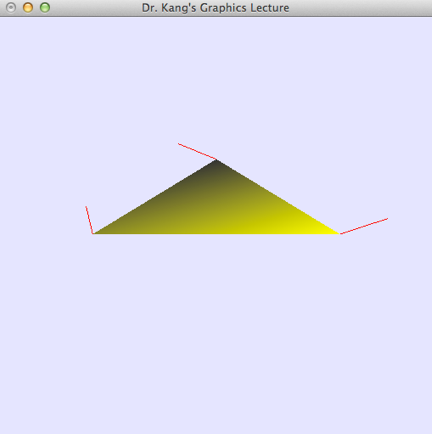
\includegraphics[height=6.5cm]{OGL_light/normalSetting.png}
\end{figure}

\end{frame}
%%%%%%%%%%%%%%%%%%%%%%%%%%%%%%%%%%%%%%%%%%%%%%%%%%%%%%%%%


%%%%%%%%%%%%%%%%%%%%%%%%%%%%%%%%%%%%%%%%%%%%%%%%%%%%%%%%%
\begin{frame}[fragile]{구로 세이딩 - 두 개의 인접한 면 그리기}

\lstset{language=C++, escapechar=^} 
\begin{lstlisting}
  glBegin(GL_TRIANGLES);
  glNormal3f(-1/sqrt(2),1/sqrt(2),0);
  glVertex3f(0,1,0);
  glVertex3f(-1,0,0);
  glVertex3f(0,1,1);
  glNormal3f(1/sqrt(2),1/sqrt(2),0);
  glVertex3f(0,1,0);
  glVertex3f(0,1,1);
  glVertex3f(1,0,0);
  glEnd();
\end{lstlisting}

\begin{figure}[h!]
  \centering
    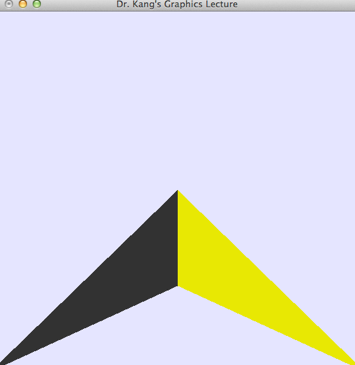
\includegraphics[height=4.5cm]{OGL_light/twoFacesTwoNormals.png}
\end{figure}

\end{frame}
%%%%%%%%%%%%%%%%%%%%%%%%%%%%%%%%%%%%%%%%%%%%%%%%%%%%%%%%%

%%%%%%%%%%%%%%%%%%%%%%%%%%%%%%%%%%%%%%%%%%%%%%%%%%%%%%%%%
\begin{frame}[fragile]{구로 세이딩 - 법선 벡터 공유하기}

\lstset{language=C++, escapechar=^} 
\begin{lstlisting}
  glBegin(GL_TRIANGLES);
  glNormal3f(0,1,0);  
  glVertex3f(0,1,0);
  glNormal3f(-1/sqrt(2),1/sqrt(2),0);  
  glVertex3f(-1,0,0);
  glNormal3f(0,1,0);  
  glVertex3f(0,1,1);
  glNormal3f(0,1,0);  
  glVertex3f(0,1,0);
  glNormal3f(0,1,0);  
  glVertex3f(0,1,1);
  glNormal3f(1/sqrt(2),1/sqrt(2),0);  
  glVertex3f(1,0,0);
  glEnd();
\end{lstlisting}

\begin{figure}[h!]
  \centering
    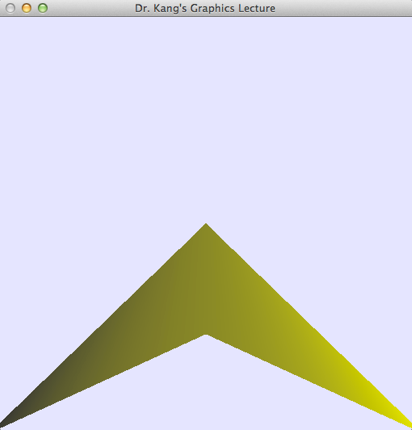
\includegraphics[height=4.0cm]{OGL_light/twoFacesFourNormals.png}
\end{figure}

\end{frame}
%%%%%%%%%%%%%%%%%%%%%%%%%%%%%%%%%%%%%%%%%%%%%%%%%%%%%%%%%

%%%%%%%%%%%%%%%%%%%%%%%%%%%%%%%%%%%%%%%%%%%%%%%%%%%%%%%%%
\begin{frame}[fragile]{구로 세이딩 - 법선 벡터 공유하기}

\lstset{language=C++, escapechar=^} 
\begin{lstlisting}
  glBegin(GL_TRIANGLES);
  glNormal3f(0,1,0);  
  glVertex3f(0,1,0);
  glNormal3f(-1/sqrt(2),1/sqrt(2),0);  
  glVertex3f(-1,0,0);
  glNormal3f(0,1,0);  
  glVertex3f(0,1,1);
  glNormal3f(0,1,0);  
  glVertex3f(0,1,0);
  glNormal3f(0,1,0);  
  glVertex3f(0,1,1);
  glNormal3f(1/sqrt(2),1/sqrt(2),0);  
  glVertex3f(1,0,0);
  glEnd();
\end{lstlisting}

\begin{figure}[h!]
  \centering
    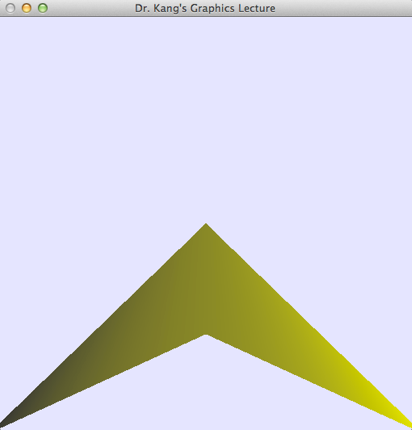
\includegraphics[height=4.0cm]{OGL_light/twoFacesFourNormals.png}
\end{figure}

\end{frame}
%%%%%%%%%%%%%%%%%%%%%%%%%%%%%%%%%%%%%%%%%%%%%%%%%%%%%%%%%


%%%%%%%%%%%%%%%%%%%%%%%%%%%%%%%%%%%%%%%%%%%%%%%%%%%%%%%%%
\begin{frame}[fragile]{메시(mesh)}

\begin{table}
\caption{메시 데이터 포맷의 예시}
\label{tab:meshDataExample}
\begin{center}
    \begin{tabular}{ |l|l|}
    \hline
    {\small \sf 포맷} & {\small \sf 실제 데이터 예시} \\ \hline
numVertices $n$  & 4\\ 
vertex 1 ($x_1,y_1,z_1$) & 0.0 1.0  0.0\\ 
vertex 2 ($x_2,y_2,z_2$) & -1.0  0.0  0.0\\ 
... &  0.0  1.0  1.0\\ 
vertex $n$ ($x_n,y_n,z_n$) & 1.0  0.0  0.0\\ 
numFaces $m$ & 2\\ 
face 1 ($f_1.v_1,f_1.v_2,f_1.v_3$) &  0 1 2\\
face 2 ($f_2.v_1,f_2.v_2,f_2.v_3$) & 0 2 3\\
 ... & \\ 
\hline
\end{tabular}
\end{center}
\end{table}

\end{frame}
%%%%%%%%%%%%%%%%%%%%%%%%%%%%%%%%%%%%%%%%%%%%%%%%%%%%%%%%%


%%%%%%%%%%%%%%%%%%%%%%%%%%%%%%%%%%%%%%%%%%%%%%%%%%%%%%%%%
\begin{frame}[fragile]{메시(mesh) 로딩}

\lstset{language=C++, escapechar=^} 
\begin{lstlisting}
#ifndef _mesh_sms_hh_
#define _mesh_sms_hh_
class cvertex {
public:
    float x;
    float y;
    float z;
}; // ^{\it 하나의 점을 구성하는 좌표값 3 개}^
class cface {
public:
    int v0; int v1; int v2;
}; //^{\it 하나의 삼각형 면을 구성하는 세 개 정점의 인덱스들}^

class CMesh {
    int nV;  // ^{\it 정점의 개수}^
    int nF;  // ^{\it 메시 구성 삼각형 면의 수}^
    cvertex *v; // ^{\it 정점 데이터 배열}^
    cface   *f; // ^{\it 면 데이터 배열}^

public:
    float minx, miny, minz;
    float maxx, maxy, maxz; // ^{\it 메시를 둘러싸는 AABB 경계상자}^

public:
    CMesh();  // constructor
    ~CMesh(); // destructor
    // ^{\it 메시를 읽고 그리는 메소드들}^
    void loadMesh(char *meshFileName);
    void drawMesh(void);
};
#endif
\end{lstlisting}

\end{frame}
%%%%%%%%%%%%%%%%%%%%%%%%%%%%%%%%%%%%%%%%%%%%%%%%%%%%%%%%%


%%%%%%%%%%%%%%%%%%%%%%%%%%%%%%%%%%%%%%%%%%%%%%%%%%%%%%%%%
\begin{frame}[fragile]{메시(mesh) 로딩}

\lstset{language=C++, escapechar=^} 
\begin{lstlisting}
#include "Mesh.h" 
^{\sf [[필요한 헤더 파일들 포함]]}^
#define BIGNUMBER 100000000000000000000000.0
CMesh::CMesh() : nV(0), nF(0), v(NULL), f(NULL), minx( BIGNUMBER), miny( BIGNUMBER), minz( BIGNUMBER), maxx(-BIGNUMBER), maxy(-BIGNUMBER), maxz(-BIGNUMBER) { }

CMesh::~CMesh() {
    if(v) delete[] v;
    if(f) delete[] f;    
}
void CMesh::loadMesh(char *meshFileName) {
    FILE *fptr = fopen(meshFileName, "r");
    if(!meshFileName || !fptr) {  printf("file open error\n"); exit(0);      }
    fscanf(fptr, "%d", &nV);    // ^{\it 정점의 개수 읽기}^
    v = new cvertex[nV];
    for (int i=0; i<nV; i++) {
        // ^{\it {\sf nV}개의 정점 정보를 읽음}^
        fscanf(fptr, "%f", &v[i].x); 
        fscanf(fptr, "%f", &v[i].y); 
        fscanf(fptr, "%f", &v[i].z);
    }
    fscanf(fptr, "%d", &nF);     // ^{\it 면의 개수 읽기}^
    f = new cface[nF];
    for (int i=0; i<nF; i++) { // ^{\it {\sf nF}개의 면 정보를 읽음}^        
        fscanf(fptr, "%d", &f[i].v0);   
        fscanf(fptr, "%d", &f[i].v1);    
        fscanf(fptr, "%d", &f[i].v2);
    }
}
\end{lstlisting}

\end{frame}
%%%%%%%%%%%%%%%%%%%%%%%%%%%%%%%%%%%%%%%%%%%%%%%%%%%%%%%%%

%%%%%%%%%%%%%%%%%%%%%%%%%%%%%%%%%%%%%%%%%%%%%%%%%%%%%%%%%
\begin{frame}[fragile]{메시(mesh) 그리기 1}

\lstset{language=C++, escapechar=^} 
\begin{lstlisting}
void CMesh::drawMesh(void) {
  if(!v || !f) return;
  glBegin(GL_POINTS);
  for(int i=0;i<nV;i++) {
    glVertex3f( v[i].x, v[i].y, v[i].z);
  }
  glEnd();
}
\end{lstlisting}

\begin{figure}[h!]
  \centering
    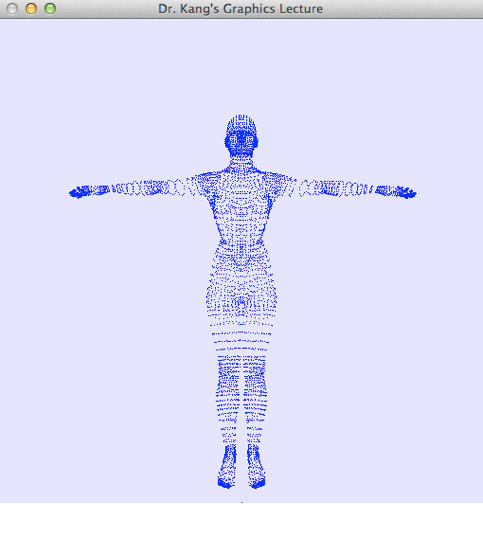
\includegraphics[height=5cm]{OGL_light/drawMeshVerts.png}
\end{figure}

\end{frame}
%%%%%%%%%%%%%%%%%%%%%%%%%%%%%%%%%%%%%%%%%%%%%%%%%%%%%%%%%

%%%%%%%%%%%%%%%%%%%%%%%%%%%%%%%%%%%%%%%%%%%%%%%%%%%%%%%%%
\begin{frame}[fragile]{메시(mesh) 그리기 2}

\lstset{language=C++, escapechar=^} 
\begin{lstlisting}
void CMesh::drawMesh(void) {
    for (int i=0; i<nF; i++) {
        // ^{\it i-번째 면을 그리는 작업}^
        int a, b, c; // ^{\it 삼각형을 구성하는 세 정점의 인덱스}^
        a = f[i].v0; // ^{\it i-번째 면의 0번 정점}^
        b = f[i].v1; // ^{\it i-번째 면의 1번 정점}^
        c = f[i].v2; // ^{\it i-번째 면의 2번 정점}^
        glBegin(GL_LINE_LOOP);
        glVertex3f(v[a].x, v[a].y, v[a].z); // ^{\it a 정점의 좌표}^
        glVertex3f(v[b].x, v[b].y, v[b].z);// ^{\it b정점의 좌표}^
        glVertex3f(v[c].x, v[c].y, v[c].z); // ^{\it c 정점의 좌표}^
        glEnd();
    }
}
\end{lstlisting}

\begin{figure}[h!]
  \centering
    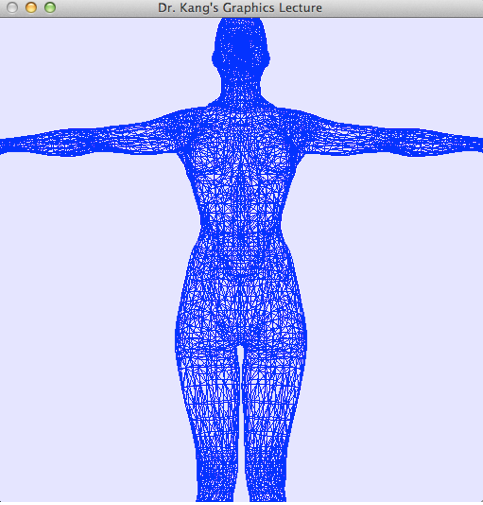
\includegraphics[height=4cm]{OGL_light/meshEdgeDraw.png}
\end{figure}

\end{frame}
%%%%%%%%%%%%%%%%%%%%%%%%%%%%%%%%%%%%%%%%%%%%%%%%%%%%%%%%%

%%%%%%%%%%%%%%%%%%%%%%%%%%%%%%%%%%%%%%%%%%%%%%%%%%%%%%%%%
\begin{frame}[fragile]{메시(mesh) 그리기 3 - 면}

\lstset{language=C++, escapechar=^} 
\begin{lstlisting}
void CMesh::drawMesh(void) {
    if(!v || !f) return;
    glBegin (GL_TRIANGLES) ; 

    for(int i=0;i<nF;i++) {
        // ^{\it 법선 벡터를 계산하기 위한 정보}^
        cvertex p0, p1, p2;  // ^{\it 세 개의 정점 ${\mathbf p}_0, {\mathbf p}_1, {\mathbf p}_2$}^
        cvertex v0, v1; cvertex n; //^{\it 면 위의 두 벡터 ${\mathbf v}_0, {\mathbf v}_1$와 법선벡터 $\mathbf n$}^
        p0 = v[f[i].v0];
        p1 = v[f[i].v1];
        p2 = v[f[i].v2];

        // ^{\it ${\mathbf v}_0 = {\mathbf p}_1 - {\mathbf p}_0$}^
        v0.x = p1.x-p0.x; v0.y = p1.y-p0.y; v0.z = p1.z-p0.z; 
        // ^{\it ${\mathbf v}_1 = {\mathbf p}_2 - {\mathbf p}_0$}^
        v1.x = p2.x-p0.x; v1.y = p2.y-p0.y; v1.z = p2.z-p0.z;

        // ^{\it ${\mathbf n} = \frac{{\mathbf v}_1 \times {\mathbf v}_0}{|{\mathbf v}_1 \times {\mathbf v}_0|}$}^
        n.x = v0.y*v1.z-v0.z*v1.y;
        n.y = v0.z*v1.x-v0.x*v1.z;
        n.z = v0.x*v1.y-v0.y*v1.x;
        float len = sqrt(n.x*n.x+n.y*n.y+n.z*n.z); 
        n.x /= len; n.y /= len; n.z /= len;

        glNormal3f(n.x, n.y, n.z); 
        glVertex3f( p0.x, p0.y, p0.z); 
        glVertex3f( p1.x, p1.y, p1.z); 
        glVertex3f( p2.x, p2.y, p2.z);
    }
    glEnd() ;
}
\end{lstlisting}


\end{frame}
%%%%%%%%%%%%%%%%%%%%%%%%%%%%%%%%%%%%%%%%%%%%%%%%%%%%%%%%%

%%%%%%%%%%%%%%%%%%%%%%%%%%%%%%%%%%%%%%%%%%%%%%%%%%%%%%%%%
\begin{frame}[fragile]{메시(mesh) 면 그리기 결과}

\begin{figure}[h!]
  \centering
    \fbox{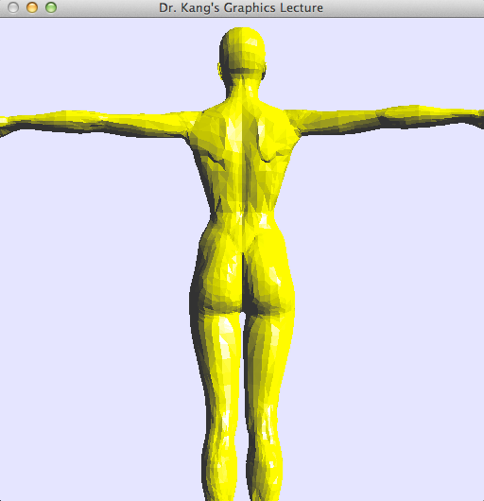
\includegraphics[height=7cm]{OGL_light/meshFlatSurfaces.png}}
\end{figure}

\end{frame}
%%%%%%%%%%%%%%%%%%%%%%%%%%%%%%%%%%%%%%%%%%%%%%%%%%%%%%%%%

%%%%%%%%%%%%%%%%%%%%%%%%%%%%%%%%%%%%%%%%%%%%%%%%%%%%%%%%%
\begin{frame}[fragile]{메시(mesh) 그리기 - 법선 벡터의 저장}

\begin{itemize}
\item 매번 면을 그릴 때마다 법선벡터를 계산하는 것은 비효율적
\item 한 번 법선 벡터를 계산한 뒤, 이 결과를 각 정점별로 저장
\end{itemize}

\lstset{language=C++, escapechar=^} 
\begin{lstlisting}
class CMesh {
    int nV;  // number of vertices
    int nF;  // number of faces
    cvertex *v; // vertex array
    cface   *f; // face array
    cvertex *n; // ^{\it \color{red} 법선 벡터의 배열}^
...
public:
...
    void computeNormals(void); // ^{\it \color{red} 법선 벡터를 계산하여 {\sf n}에 채움}^
};

#endif
\end{lstlisting}

\end{frame}
%%%%%%%%%%%%%%%%%%%%%%%%%%%%%%%%%%%%%%%%%%%%%%%%%%%%%%%%%

%%%%%%%%%%%%%%%%%%%%%%%%%%%%%%%%%%%%%%%%%%%%%%%%%%%%%%%%%
\begin{frame}[fragile]{메시(mesh) 그리기 - 법선 벡터의 계산}

\begin{itemize}
\item 입력된 데이터를 이용하여 법선 벡터를 계산하는 {\sf computeNormals} 메소드를 호출
\item {\sf computeNormals} 메소드는 앞에서 법선 벡터를 계산했던 방식과 동일한 방법으로 각각의 면에 대해 법선 {\sf N}을 계산
\item 이 법선 벡터는 바로 사용되지 않음
\item 어떤 면을 구성하는 정점이 $\mathbf p_0, \mathbf p_1, \mathbf p_2$라면 각각의 법선 벡터를 $\mathbf n_0, \mathbf n_1, \mathbf n_2$.
\item 이 면에서 얻어진 법선 벡터는 $\mathbf n_0, \mathbf n_1, \mathbf n_2$에 누적
\end{itemize}
\begin{eqnarray} \nonumber
\mathbf n_0 = \mathbf n_0 + {\mathbf N} \\ \nonumber
\mathbf n_1 = \mathbf n_1 + {\mathbf N} \\ \nonumber
\mathbf n_2 = \mathbf n_2 + {\mathbf N} \\ \nonumber
\end{eqnarray}

모든 $\mathbf n_i$에 대해 정규화를 수행하면 각 정정별 법선을 얻을 수 있다.

\end{frame}
%%%%%%%%%%%%%%%%%%%%%%%%%%%%%%%%%%%%%%%%%%%%%%%%%%%%%%%%%

%%%%%%%%%%%%%%%%%%%%%%%%%%%%%%%%%%%%%%%%%%%%%%%%%%%%%%%%%
\begin{frame}[fragile]{메시(mesh) 그리기 - 법선 벡터의 저장}

\lstset{language=C++, escapechar=^} 
\begin{lstlisting}
void CMesh::computeNormals(void) { // private method    
    for(int i=0;i<nV;i++) {
        n[i].x = n[i].y = n[i].z = 0.0;
    }    
    for(int i=0; i<nF; i++) {
        // ^{\it 각각의 면에 대해서 외적을 이용한 법선 계산을 수행한다}^
        cvertex p0, p1, p2;
        cvertex v0, v1; cvertex N;
        int vert0, vert1, vert2;
        vert0 = f[i].v0; vert1 = f[i].v1; vert2 = f[i].v2;
        p0 = v[vert0];
        p1 = v[vert1];
        p2 = v[vert2];
        v0.x = p1.x-p0.x; v0.y = p1.y-p0.y; v0.z = p1.z-p0.z;
        v1.x = p2.x-p0.x; v1.y = p2.y-p0.y; v1.z = p2.z-p0.z;        
        N.x = v0.y*v1.z-v0.z*v1.y;
        N.y = v0.z*v1.x-v0.x*v1.z;
        N.z = v0.x*v1.y-v0.y*v1.x;
        // ^{\it 이렇게 얻어진 법선 벡터는 이 면을 구성하고 있는 정점 3 개의 법선 데이터에 누적된다}^
        n[vert0].x += N.x; n[vert0].y += N.y; n[vert0].z += N.z;
        n[vert1].x += N.x; n[vert1].y += N.y; n[vert1].z += N.z;
        n[vert2].x += N.x; n[vert2].y += N.y; n[vert2].z += N.z;
    }    
    for(int i=0;i<nV;i++) {
        // ^{\it 모든 정정에 대해 누적된 법선 벡터를 정규화한다}^
        float len = sqrt(n[i].x*n[i].x+n[i].y*n[i].y+n[i].z*n[i].z);
        n[i].x /= len; n[i].y /= len; n[i].z /= len;
    }    
}
#endif
\end{lstlisting}

\end{frame}
%%%%%%%%%%%%%%%%%%%%%%%%%%%%%%%%%%%%%%%%%%%%%%%%%%%%%%%%%

%%%%%%%%%%%%%%%%%%%%%%%%%%%%%%%%%%%%%%%%%%%%%%%%%%%%%%%%%
\begin{frame}[fragile]{메시(mesh) 그리기 - 렌더링 결과}

\begin{figure}[h!]
  \centering
    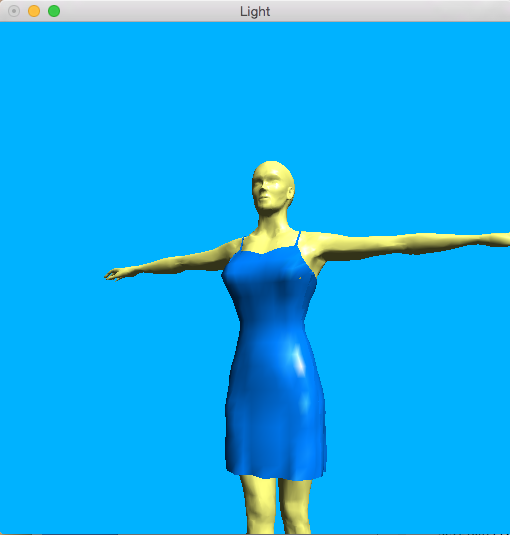
\includegraphics[height=7cm]{OGL_light/meshSmoothSurfaces.png}
\end{figure}

\end{frame}
%%%%%%%%%%%%%%%%%%%%%%%%%%%%%%%%%%%%%%%%%%%%%%%%%%%%%%%%%

\end{document}


\section{}


